\documentclass[12pt]{article}
 
\usepackage[margin=1in]{geometry} 
\usepackage{amsmath,amsthm,amssymb}
\usepackage{graphicx}
\graphicspath{{./images/}}
 
\newcommand{\N}{\mathbb{N}}
\newcommand{\Z}{\mathbb{Z}}
 
\newenvironment{theorem}[2][Theorem]{\begin{trivlist}
\item[\hskip \labelsep {\bfseries #1}\hskip \labelsep {\bfseries #2.}]}{\end{trivlist}}
\newenvironment{lemma}[2][Lemma]{\begin{trivlist}
\item[\hskip \labelsep {\bfseries #1}\hskip \labelsep {\bfseries #2.}]}{\end{trivlist}}
\newenvironment{exercise}[2][Exercise]{\begin{trivlist}
\item[\hskip \labelsep {\bfseries #1}\hskip \labelsep {\bfseries #2.}]}{\end{trivlist}}
\newenvironment{reflection}[2][Reflection]{\begin{trivlist}
\item[\hskip \labelsep {\bfseries #1}\hskip \labelsep {\bfseries #2.}]}{\end{trivlist}}
\newenvironment{proposition}[2][Proposition]{\begin{trivlist}
\item[\hskip \labelsep {\bfseries #1}\hskip \labelsep {\bfseries #2.}]}{\end{trivlist}}
\newenvironment{corollary}[2][Corollary]{\begin{trivlist}
\item[\hskip \labelsep {\bfseries #1}\hskip \labelsep {\bfseries #2.}]}{\end{trivlist}}
 
\begin{document}
 
% --------------------------------------------------------------
%                         Start here
% --------------------------------------------------------------
 
%\renewcommand{\qedsymbol}{\filledbox}
 
\title{Physics Tutoring Practice Problems}%replace X with the appropriate number
\author{Christian Parizeau\\ %replace with your name
Electro and Magneto Statics} %if necessary, replace with your course title
 
\maketitle
\section{Overview}
This is the first installment in a series of extra practice problems to be completed throughout the year. This assignment will cover Gauss' Law, capacitors and resistors as circuit elements, and electrostatic potential. While this assignment is review to help solidify concepts before your exam, future assignments will include more problems that are outside of your comfort zone. If you don't know how to solve any of the problems, that's ok! These are not meant to be solved in a vacuum, please use any resource you can to solve these problems. And if you still can't work out the problems, come to me and we'll work it through together. \\\\
1) Two conducting sphere are concentrically nested. The inner sphere has a radius of $3$cm and a net charge of $12\mu$C. The outer spherical shell has an inner radius of $6$cm, an outer radius of $8$cm, and a net charge of $-6\mu$C. Determine the net  charge on the inner surface of the outer spherical shell, on the outer surface of the outer spherical shell. As well as the electric field strength and magnitude in each unique region (from the center of the inner sphere, to outside both spheres).
\\\\\\\\\\\\\\\\\\\\\\\\\\\\\\\\\\\
2) Determine the current through and voltage drop across each resistor in the diagram. \\
\begin{figure}[h]
    \centering
    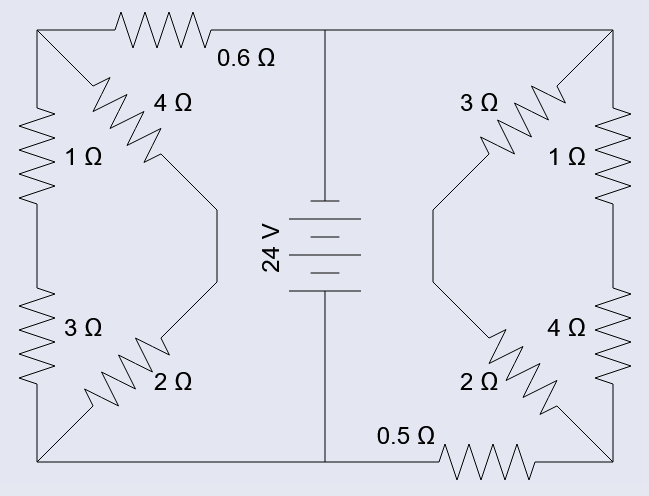
\includegraphics{images/resistorCircuit.PNG}
    \caption{Hint: Can you identify which resistors are in parallel and which are in seris?}
    \label{fig:my_label}
\end{figure}
\\\\\\\\\\\\\\\\\\\\\\\\\\\\
3) Calculate the equivalent capacitance of the diagram below
\begin{figure}[h]
    \centering
    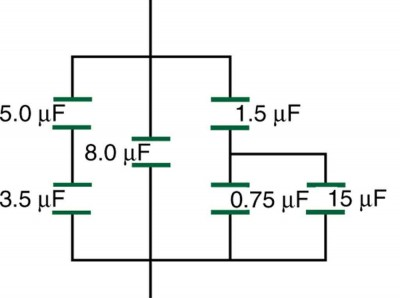
\includegraphics{images/capcacitors.jpg}
    
    \label{fig:my_label}
\end{figure}
\\\\\\\\\\\\\\\\\\\\\\\
4) 4 identical point charges (of charge $+1\mu$C) are placed at the 4 vertices of a square (side length $\sqrt{2}$. Find the electric potential at the center, and 4 meters directly above the middle of the square. 
% --------------------------------------------------------------
%     You don't have to mess with anything below this line.
% --------------------------------------------------------------
 
\end{document}